% Chapter 1 - Introduction to Monsoon-Driven Crop Price Prediction
\chapter{Introduction to Monsoon-Driven Crop Price Prediction}

India's agricultural economy is intricately tied to the monsoon, which directly impacts the yield and market value of Kharif crops \cite{gadgil2006monsoon, sarkar2019monsoon}. This chapter introduces the motivation behind developing a predictive system for crop prices influenced by seasonal rainfall trends. It outlines the context and importance of the project, defines the specific problem being addressed, and clearly states the objectives of the work. In addition, it presents an overview of the methodology used, the assumptions made during implementation, and the structure of the report that follows.

\section[Introduction]{\textbf{Introduction}}

Agriculture forms the backbone of the Indian economy, with a significant portion of the population relying on farming for their livelihood \cite{birthal2015}. Among the different cropping seasons, the Kharif season is particularly crucial, as it is heavily dependent on the monsoon \cite{gadgil2006monsoon}. The unpredictability of rainfall directly influences crop yields and, consequently, the market prices of essential commodities like rice, maize, and pulses \cite{ray2019climate}. Price volatility creates uncertainty for farmers and buyers alike, making it difficult to plan cultivation and trading activities effectively \cite{timmer2009price}.

To address this issue, the project titled \textit{Monsoon-Driven Crop Price Prediction} aims to forecast the prices of Kharif crops based on historical data trends and regional inputs. By leveraging government-sourced datasets and applying machine learning techniques, the project seeks to offer a reliable price prediction tool through an interactive web interface. This system not only predicts future prices but also visualizes past pricing patterns, empowering farmers, traders, and policymakers with valuable insights for decision-making \cite{jain2020deep, mahmud2025price}.

\begin{comment}
	You are allowed to use figures or diagrams which can help in introducing the topic acknowledging the source. For example, if you are introducing a particular topic, an appropriate figure can be used. The figure should be referenced in the text as Figure~\ref{fig:universe}.
	
	\begin{figure}[H]
		\centering
		
\includegraphics[scale=0.4]{Figures/universe}
		\caption{Sample picture of universe}
		\label{fig:universe}
	\end{figure}
\end{comment}

%These guidelines are provided to formally expose you to the various ethical %and technical issues involved in writing up your work and the format you are %required to adhere to while submitting your project report.
\section[Literature Review]{\textbf{Literature Review}}

This section reviews relevant academic contributions in the domain of crop price and yield prediction, with a focus on monsoon-related variability and regional forecasting models in India. The reviewed works span multiple methodologies including machine learning, deep learning, statistical modeling, and remote sensing. These papers collectively emphasize the importance of using climate data, particularly monsoon characteristics, in building reliable, region-specific price or yield prediction systems for agricultural decision-making.

\subsection{Impact of COVID-19 on Indian Agriculture \cite{cariappa2020impact}}
Cariappa et al. (2020) provide an extensive analysis of the COVID-19 pandemic's effects on Indian agriculture, underscoring how pre-existing systemic issues were amplified during the crisis. The paper outlines the consequences of nationwide lockdowns on supply chain dynamics, market accessibility, and price stability. In particular, farmers faced significant difficulties in transporting produce, accessing inputs, and finding buyers, which led to large post-harvest losses and income instability. The study makes special mention of the disproportionate impact on smallholder farmers who lacked digital tools or access to storage infrastructure. Using state-wise case studies, including Karnataka, the paper reveals stark differences in market recovery speeds and resilience. The researchers advocate for the creation of robust digital platforms to enable real-time access to market and weather information. This resonates directly with our project's goals, emphasizing the need for predictive tools that not only mitigate monsoon-driven variability but also serve as a buffer during unprecedented disruptions. By presenting a holistic view of agricultural vulnerabilities under extreme conditions, the study sets a strong contextual foundation for our work.

\subsection{Price Forecasting with LSTM Networks \cite{mahmud2025price}}
Mahmud et al. (2025) present a detailed examination of LSTM-based forecasting models applied to agricultural commodity prices across India, emphasizing their effectiveness in handling temporal dependencies and nonlinearities in pricing data. The paper explores multiple variants of LSTM, comparing their performance to classical statistical models like ARIMA and Holt-Winters on commodities such as rice and pulses. A standout feature of the research is the inclusion of exogenous climatic factors like rainfall, humidity, and temperature as input variables, which significantly enhanced prediction accuracy. The authors validate their findings using datasets from multiple Indian states, ensuring model robustness and generalizability. The results show that LSTM-based models consistently outperform traditional models, especially during periods of sudden climatic variability. The study concludes with recommendations for integrating these models into real-time decision support systems. For our project focused on Karnataka's Kharif crops, this paper provides not only methodological inspiration but also empirical validation for incorporating deep learning models that leverage climatic indicators. The emphasis on combining temporal modeling with external variables strengthens the rationale behind our design choices.

\subsection{Yield Forecasting Using ML in Karnataka \cite{kumar2024yield}}
Kumar et al. (2024) investigate the application of machine learning algorithms—specifically Random Forest and Support Vector Regression (SVR)—for rice yield forecasting in Karnataka. The study sources data from government repositories, comprising over a decade of observations on rainfall, humidity, temperature, soil characteristics, and cropping patterns. Through rigorous training and validation, Random Forest emerged as the most accurate and stable model, demonstrating an ability to capture complex nonlinear interactions between variables. The researchers emphasize the importance of district-level models due to Karnataka's diverse agro-climatic zones, noting that state-aggregated models often overlook local nuances. Their work highlights the need for granular data and localized analysis, especially in contexts where regional variability can significantly alter agricultural outcomes. Additionally, the study provides a practical framework for integrating environmental and soil data into predictive systems. While the research focuses on yield rather than price, the insights into spatial modeling, feature importance, and model scalability are directly transferable to our project. This alignment supports our emphasis on region-specific forecasting and further justifies our methodological focus.

\subsection{ARIMA-Based Forecasting of Agri Prices \cite{darekar2018price}}
Darekar and Reddy (2018) offer a methodical evaluation of ARIMA models for forecasting agricultural commodity prices, drawing on a rich dataset from government procurement centers and wholesale markets. The authors focus on commodities such as onions, rice, and wheat, examining price trends over a multi-year period to assess model robustness across seasonal and economic cycles. They highlight that ARIMA performs well in capturing long-term trends and cyclical patterns but struggles with abrupt changes caused by unpredictable events like policy shifts, climate anomalies, or supply disruptions. The study advocates for hybrid forecasting systems that combine ARIMA's strengths with machine learning's adaptability. In terms of model evaluation, metrics like RMSE and MAPE are used to compare predictive accuracy, and the paper thoroughly documents preprocessing steps such as stationarity testing and parameter tuning. While ARIMA serves as a solid baseline, the study concludes that dynamic, learning-based models are more suited for volatile environments like India's agri-markets. This underscores our decision to integrate monsoon variables and machine learning algorithms, using ARIMA results as a performance benchmark for more advanced models.

\subsection{Machine Learning in Crop Yield Forecasting \cite{ghetiya2024ml}}
Ghetiya et al. (2024) provide a comprehensive overview and empirical evaluation of machine learning techniques—including Decision Trees, Random Forest, and XGBoost—for yield forecasting in Indian agriculture. The dataset spans 15 years and includes information on climate, soil properties, seed quality, and market inputs. The study conducts experiments across different agro-climatic regions and reports that XGBoost delivers the highest predictive accuracy, particularly in scenarios involving variable rainfall and fertilizer use. The authors make a compelling case for multi-source data integration, citing improved generalization and model reliability. A noteworthy aspect is their discussion on feature selection, where agro-meteorological indicators are consistently ranked as the most impactful variables. The paper also emphasizes the importance of regional customization, suggesting that even within a single state, model tuning can significantly improve outcomes. Though it does not tackle price forecasting directly, the insights into feature importance and algorithmic performance provide a strong foundation for our work. This study reaffirms our choice of ensemble models and justifies the attention we give to regional data segmentation in our project.

\subsection{CNN-LSTM for Crop Price Prediction \cite{ragunath2025cnn}}
Ragunath and Rathipriya (2025) propose a novel deep learning architecture that combines Convolutional Neural Networks (CNN) with Long Short-Term Memory (LSTM) networks to forecast crop prices. The model is trained on a comprehensive dataset that includes temporal price data, regional climate information, and spatial cropping patterns. The CNN component is used to extract regional features such as district-level cropping intensity and market access, while the LSTM component captures temporal dependencies and price fluctuations over time. The hybrid architecture shows significant improvements over standalone CNN or LSTM models, achieving lower error rates in MAPE and RMSE evaluations. The authors argue that combining spatial and temporal modeling better reflects the multifactorial nature of agricultural pricing, particularly in a monsoon-dependent state like Karnataka. Their study supports our design philosophy of integrating both geographic and temporal factors to create a more robust and context-aware prediction tool. Furthermore, the emphasis on model interpretability and real-world deployment makes this work a valuable reference for implementing our predictive web interface.

\subsection{Spatial Crop Suitability Mapping \cite{tripathi2021mapping}}
Tripathi et al. (2021) conduct a spatial suitability assessment of Kharif crops across Karnataka using Geographic Information System (GIS) techniques integrated with machine learning classifiers. The paper leverages extensive environmental datasets, including rainfall, temperature, soil type, and past cropping patterns, to develop suitability indices for different crops. These indices help identify optimal regions for specific crops, revealing ecological constraints and opportunities. A key insight is the correlation between ecological suitability and market price volatility—regions with lower suitability often exhibit unstable prices due to inconsistent yields. While the study does not perform direct price predictions, it provides an essential ecological baseline that enhances the explanatory power of any price prediction model. The mapping outputs are also useful for policymakers and agricultural extension officers aiming to promote climate-resilient agriculture. By contextualizing market outcomes within ecological feasibility, the paper aligns well with our project's objective of offering region-specific crop price forecasts grounded in environmental data.

\subsection{Rainfall Variability in Karnataka \cite{henrich2020rainfall}}
Henrich et al. (2020) analyze rainfall patterns in southern Karnataka over a period of 60 years to uncover long-term trends and emerging anomalies. Using data from the India Meteorological Department, the authors identify shifts in the onset, duration, and intensity of the monsoon season. Their statistical approach involves time series decomposition, anomaly detection, and spatial clustering, which reveal increased variability and delayed monsoon onset in recent decades. These findings have profound implications for agricultural planning and price forecasting, as delayed rainfall affects sowing times, yield cycles, and subsequently, market supply. The paper calls for adaptive agricultural practices and better forecasting tools that can integrate real-time weather updates. For our project, the relevance lies in using these rainfall trends as predictive features in our machine learning models. The study lends empirical support to the hypothesis that monsoon variability is a key determinant of crop price fluctuations in Karnataka.

\subsection{AI-Based Advisory Platform for Farmers \cite{singh2024ai}}
Singh and Sindhu (2024) describe the development of an AI-driven advisory system designed to assist farmers in real-time decision-making related to crop choice, irrigation scheduling, and market pricing. The platform integrates multiple data streams, including weather forecasts, soil health data, and market trends, to provide personalized recommendations. Built using ensemble machine learning techniques and designed for low-bandwidth environments, the tool is accessible via smartphones and feature phones. User studies conducted in rural districts of Haryana and Maharashtra show a marked improvement in input optimization and yield outcomes. While the system's primary goal is not price forecasting, its architecture demonstrates the feasibility and value of integrating diverse data sources into a single user interface. The emphasis on usability, accessibility, and region-specific customization offers critical lessons for our project's web application. It validates the need for user-centric design and supports the inclusion of real-time, adaptive analytics in agricultural decision support systems.

\subsection{Deep Learning for Commodity Price Forecasting \cite{jain2020deep}}
Jain et al. (2020) conduct a comprehensive evaluation of deep learning models for predicting daily commodity prices in India, focusing on LSTM, GRU, and BiLSTM architectures. The authors collect high-frequency price data from Agmarknet for rice, wheat, and pulses and compare the models across multiple error metrics. BiLSTM consistently delivers the best results due to its ability to consider both past and future contexts during training. The study also includes a detailed analysis of data preprocessing techniques like normalization, outlier treatment, and time-step optimization, all of which significantly impact model performance. Importantly, the paper discusses deployment strategies, recommending cloud-based solutions for scalability and real-time accessibility. For our project, this research offers a solid foundation in neural architecture selection, hyperparameter tuning, and deployment considerations. It reinforces our decision to use deep learning for time-series price forecasting and provides actionable insights into building a robust and scalable prediction engine.

\section[Motivation]{\textbf{Motivation}}

Agriculture continues to play a vital role in Karnataka's economy, employing a significant portion of the rural population and contributing substantially to the state's GDP \cite{niti2024, kgisac2023}. However, the cultivation and pricing of Kharif crops are highly sensitive to the onset, distribution, and intensity of the monsoon \cite{prasanna2014, gadgil2006monsoon}. In recent years, erratic rainfall patterns have made it increasingly difficult for farmers to anticipate crop yields and market prices \cite{prasanna2014, reuters_mon2025}. This uncertainty affects not only their income but also influences decisions on sowing, input purchases, and marketing strategies.

Although Karnataka has made progress in digital agriculture through various government initiatives, there is still a lack of localized, data-driven tools that can assist farmers in planning around price trends \cite{niti2024_gov}. Most existing solutions are either too generalized or inaccessible to grassroots users. This project aims to address this gap by focusing specifically on Karnataka, using its historical crop price data and regional characteristics to build a system capable of predicting prices and visualizing trends. The motivation is to empower farmers with actionable insights that reduce dependency on middlemen and speculative pricing, ultimately contributing to better financial outcomes and more sustainable agricultural practices in the state.

\section[Problem Statement]{\textbf{Problem Statement}}

Kharif crop prices in Karnataka exhibit significant seasonal and regional variability, largely influenced by unpredictable monsoon patterns and inconsistent market conditions \cite{prasanna2014, gadgil2006monsoon, henrich2020rainfall}. Farmers often lack access to timely and accurate information on future price trends, making it difficult for them to make informed decisions regarding crop selection, harvesting, and selling \cite{cariappa2020impact, jain2020deep}. This leads to financial uncertainty, exploitation by intermediaries, and inefficient resource allocation \cite{singh2024ai, niti2024}. Despite the availability of historical data, there is currently no localized, accessible platform that leverages this information to predict crop prices in a user-friendly manner \cite{tripathi2021mapping, mahmud2025price}. The problem addressed by this project is the need for a predictive and visual tool that can forecast Kharif crop prices based on time and location inputs, helping stakeholders make better decisions aligned with climatic and market realities in Karnataka.

\section[Objectives]{\textbf{Objectives}}
The objectives of the project are:
\begin{enumerate}
	\item To collect, clean, and integrate historical crop price and monsoon data specific to Karnataka from various government sources.
	\item To develop a machine learning model that predicts Kharif crop prices based on temporal and regional parameters.
	\item To build an interactive website that allows users to visualize past trends and view predicted prices based on selected time and area.
\end{enumerate}

\section[Brief Methodology of the project]{\textbf{Brief Methodology of the project}}

The overall workflow of the project is organized into multiple interdependent phases: Data Processing, ML Engineering, Development, Deployment, and User Interaction. It begins with collecting and pre-processing data related to Kharif crop prices and monsoon trends. This cleaned data is then used to develop and evaluate machine learning models in the ML Engineering Phase. Once a suitable model is finalized, it is integrated into a web application during the Development Phase. The application undergoes testing before being deployed for production use. End users can interact with the interface to obtain price predictions and visualize historical trends. A feedback loop from the user interface to the model training helps in improving future predictions.

\begin{figure}[H]
	\centering
	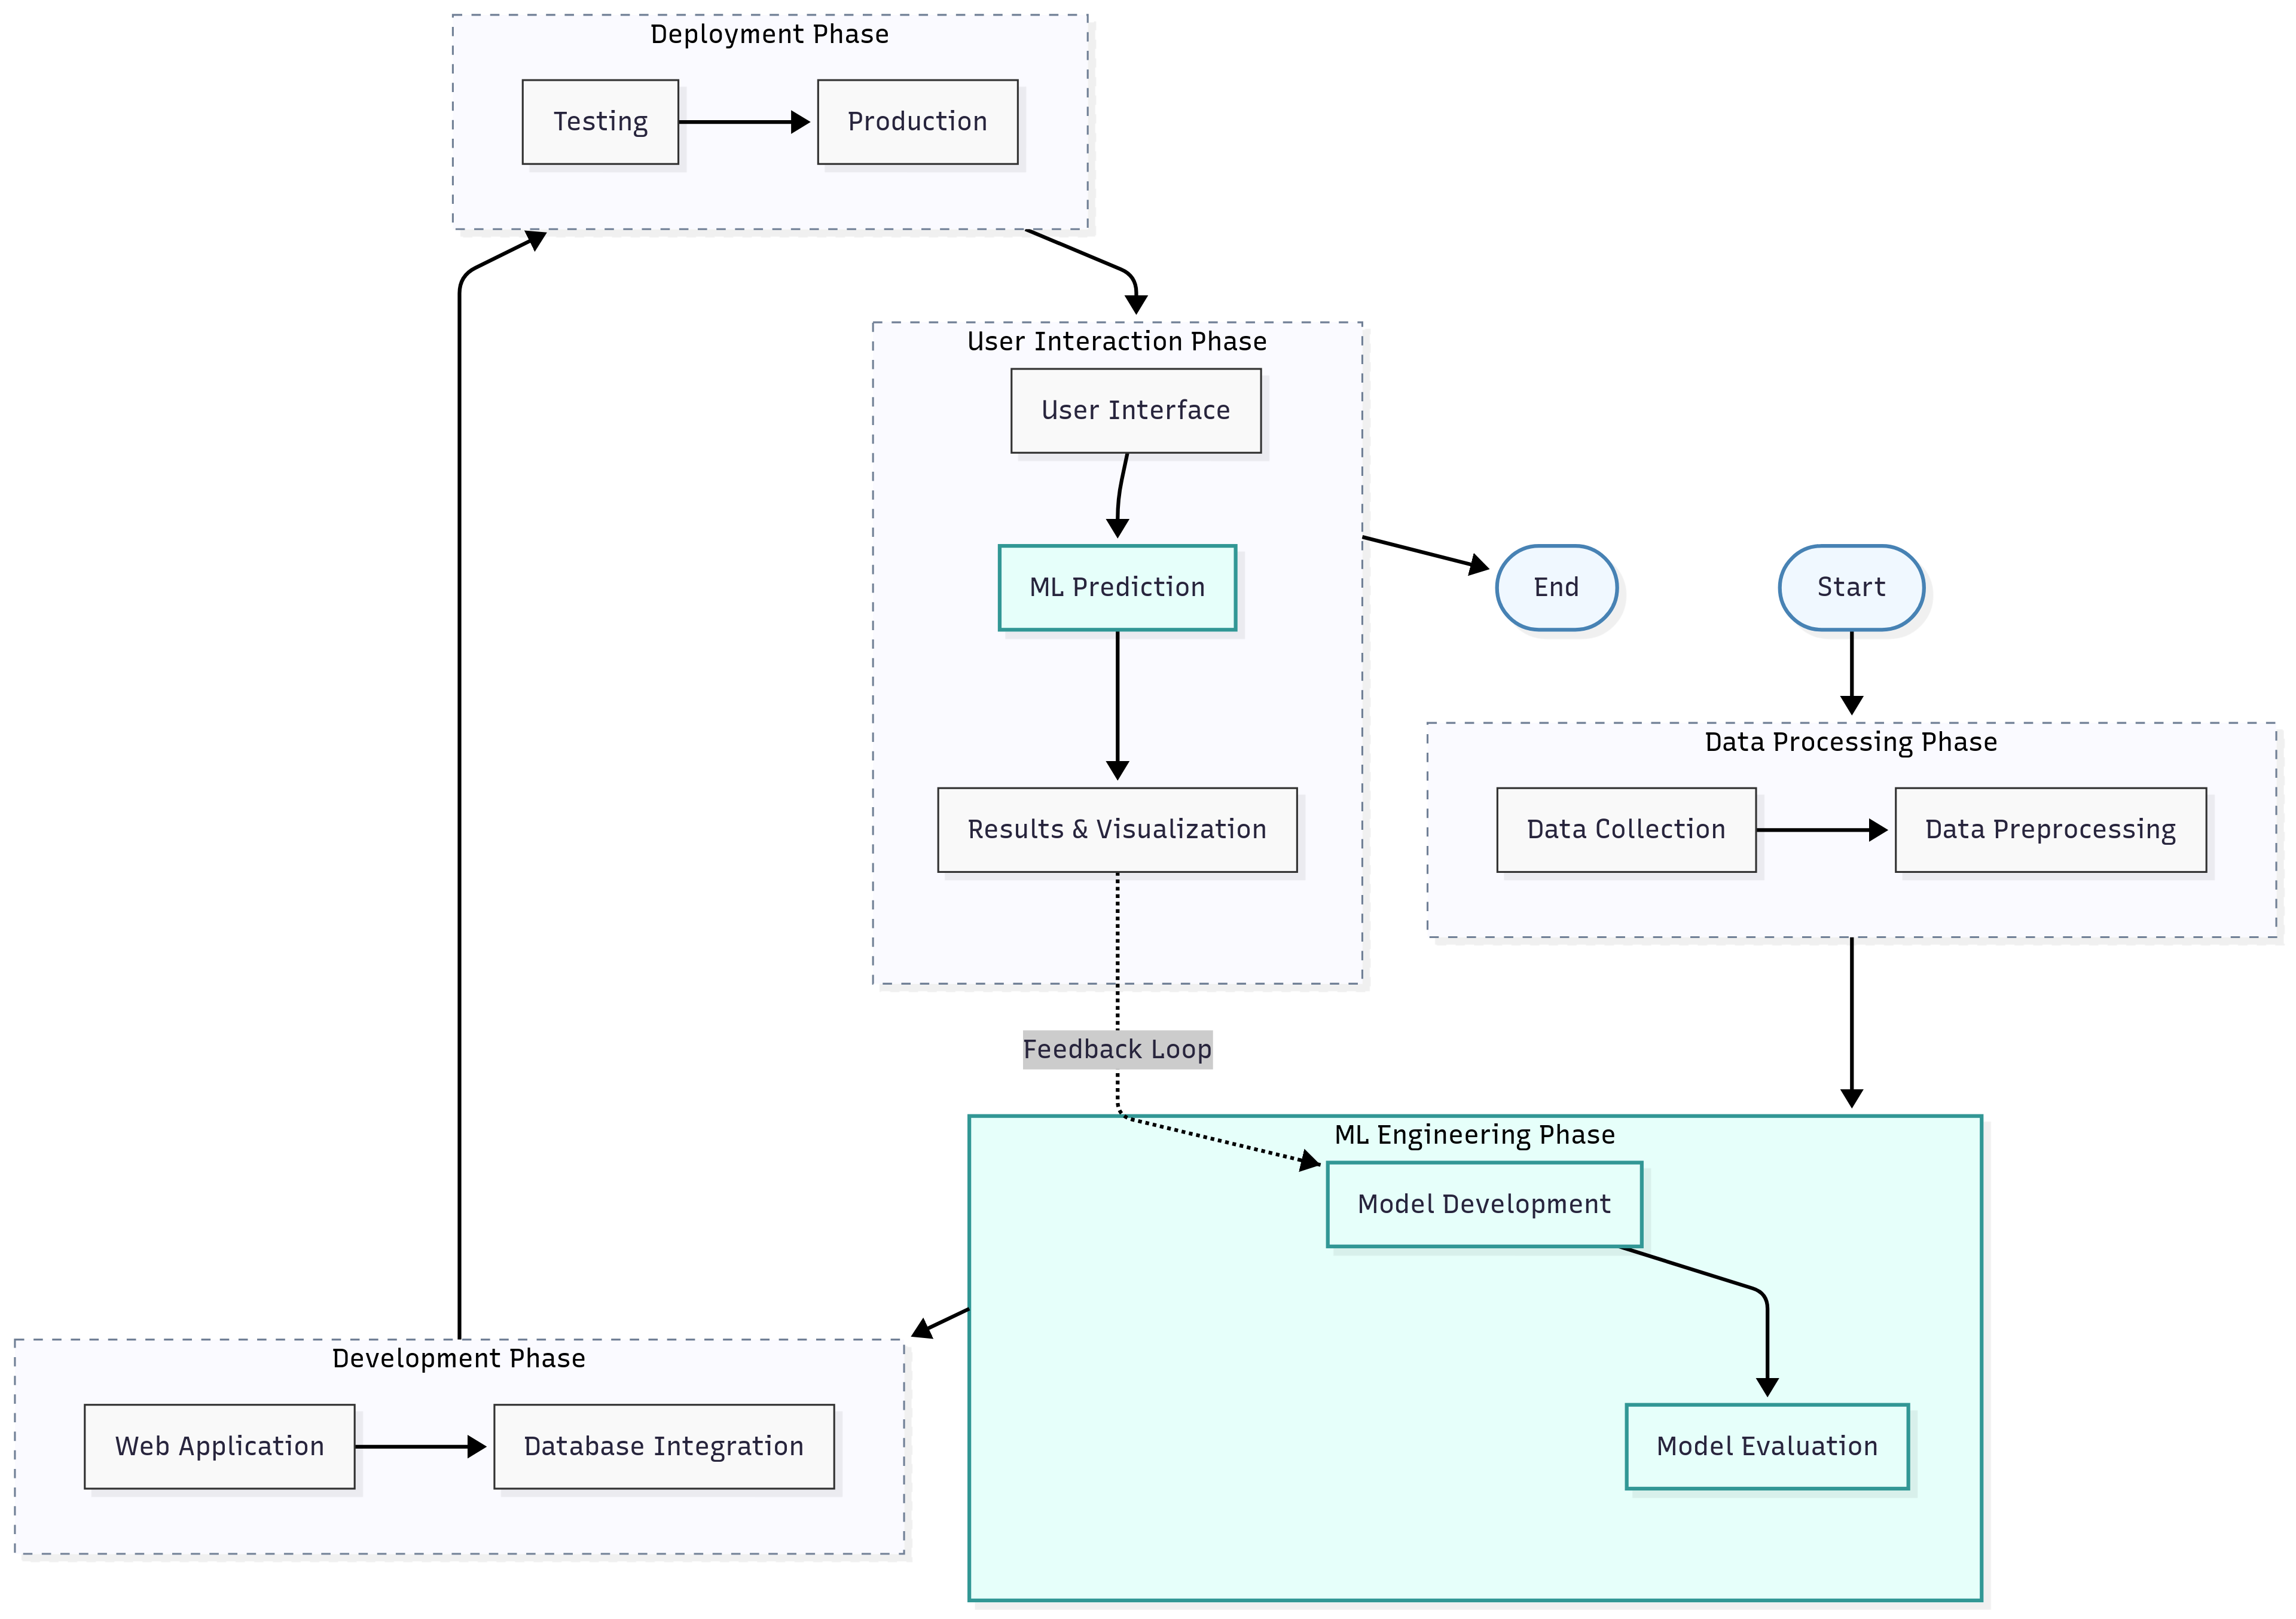
\includegraphics[width=0.95\textwidth]{Figures/Methodology_IDP.png}
	\caption{Overall Methodology of the Monsoon-Driven Crop Price Prediction System}
	\label{fig:methodology}
\end{figure}

\section[Assumptions made / Constraints of the project]{\textbf{Assumptions made / Constraints of the project}}

The following assumptions and constraints were considered during the development of the project:

\begin{itemize}
	\item It is assumed that the historical crop price data collected from government sources is accurate, reliable, and representative of market conditions across Karnataka.
	\item The model assumes that past price trends and monsoon patterns can be used as predictive indicators for future prices, with minimal interference from unexpected external events such as policy changes, natural disasters, or sudden market shocks.
	\item It is assumed that the administrative boundaries and area classifications used in the dataset remain consistent over time for valid regional comparisons.
	\item A major constraint of the project is the limited availability and granularity of historical data for some regions and crops, which may affect the precision of predictions in those areas.
	\item The current scope of the project is limited to the state of Karnataka and primarily focuses on Kharif crops; extension to other states or crop seasons would require significant data restructuring and retraining of the model.
	\item The model does not currently account for non-climatic factors such as storage costs, transportation, government subsidies, or market interventions which can also influence crop prices.
\end{itemize}

\section[Organization of the report]{\textbf{Organization of the report}}

This report is organized as follows:
\begin{itemize}
	\item Chapter 2 discusses the prerequisite theory and fundamentals required for the execution of the project.
	\item Chapter 3 discusses the AI-driven design of a scalable platform that delivers real-time insights on crop loss, price trends, and profitability to farmers.
	\item Chapter 4 discusses the implementation of the project highlighting the methodology and the technologies used.
	\item Chapter 5 discusses outcome of crop price prediction system, enabling informed agricultural decisions through analytics and visualizations.
	\item Chapter 6 discusses the comparison between the objectives and the results obtained with potential future improvements and learning outcomes.
\end{itemize}